%%% The main file. It contains definitions of basic parameters and includes all other parts.

%% Settings for single-side (simplex) printing
% Margins: left 40mm, right 25mm, top and bottom 25mm
% (but beware, LaTeX adds 1in implicitly)
\documentclass[12pt,a4paper]{report}
\setlength\textwidth{145mm}
\setlength\textheight{247mm}
\setlength\oddsidemargin{15mm}
\setlength\evensidemargin{15mm}
\setlength\topmargin{0mm}
\setlength\headsep{0mm}
\setlength\headheight{0mm}
% \openright makes the following text appear on a right-hand page
\let\openright=\clearpage
\linespread{1.25}

%% Settings for two-sided (duplex) printing
% \documentclass[11pt,a4paper,twoside,openright]{report}
% \setlength\textwidth{145mm}
% \setlength\textheight{247mm}
% \setlength\oddsidemargin{14.2mm}
% \setlength\evensidemargin{0mm}
% \setlength\topmargin{0mm}
% \setlength\headsep{0mm}
% \setlength\headheight{0mm}
% \let\openright=\cleardoublepage

%% Character encoding: usually latin2, cp1250 or utf8:
\usepackage[utf8]{inputenc}
\usepackage[svgnames,table]{xcolor}  % typesetting in color
%% Generate PDF/A-2u
\usepackage[a-2u]{pdfx}
%% Prefer Latin Modern fonts
\usepackage{lmodern}

%% Further useful packages (included in most LaTeX distributions)
\usepackage{amsmath}        % extensions for typesetting of math
\usepackage{amsfonts}       % math fonts
\usepackage{amsthm}         % theorems, definitions, etc.
%\usepackage{bbding}         % various symbols (squares, asterisks, scissors, ...)
\usepackage{bm}             % boldface symbols (\bm)
\usepackage{graphicx}       % embedding of pictures
\usepackage{fancyvrb}       % improved verbatim environment
\usepackage[square,sort,comma,numbers]{natbib}         % citation style AUTHOR (YEAR), or AUTHOR [NUMBER]
\usepackage[nottoc]{tocbibind} % makes sure that bibliography and the lists
			    % of figures/tables are included in the table
			    % of contents
\usepackage{dcolumn}        % improved alignment of table columns
\usepackage{booktabs}       % improved horizontal lines in tables
\usepackage{paralist}       % improved enumerate and itemize

\usepackage{multirow}

\usepackage{listings}
\usepackage{subcaption}
\usepackage{setspace}


%%% Basic information on the thesis

% Thesis title in English (exactly as in the formal assignment)
\def\ThesisTitleAJ{Use of residue-level annotations for structural prediction of protein-ligand binding sites}
\def\ThesisTitleCJ{Využití anotací primární struktury pro strukturní predikci protein-ligand aktivních míst}

% Author of the thesis
\def\ThesisAuthor{Kateřina Břicháčková}

% Year when the thesis is submitted
\def\YearSubmitted{2020}

% Name of the department or institute, where the work was officially assigned
% (according to the Organizational Structure of MFF UK in English,
% or a full name of a department outside MFF)
\def\Department{Katedra buněčné biologie}

% Is it a department (katedra), or an institute (ústav)?
\def\DeptType{Department}

% Thesis supervisor: name, surname and titles
\def\Supervisor{RNDr. David Hoksza, Ph.D.}


% Study programme and specialization
\def\StudyProgramme{Bioinformatics}
\def\StudyBranch{Bioinformatics}

% An optional dedication: you can thank whomever you wish (your supervisor,
% consultant, a person who lent the software, etc.)
\def\DedicationAJ{%

}

\def\DedicationCJ{%


}

% Abstract (recommended length around 80-200 words; this is not a copy of your thesis assignment!)
\def\AbstractAJ{%
abstract
}

\def\AbstractCJ{%
abstract
}

% 3 to 5 keywords (recommended), each enclosed in curly braces
\def\KeywordsAJ{%
{keyword1,} {keyword2}
}

\def\KeywordsCJ{% 
{keyword1,} {keyword2}
}

%% The hyperref package for clickable links in PDF and also for storing
%% metadata to PDF (including the table of contents).
%% Most settings are pre-set by the pdfx package.
\hypersetup{unicode}
\hypersetup{breaklinks=true}

% Definitions of macros (see description inside)
%%% This file contains definitions of various useful macros and environments %%%
%%% Please add more macros here instead of cluttering other files with them. %%%

%%% Minor tweaks of style

% These macros employ a little dirty trick to convince LaTeX to typeset
% chapter headings sanely, without lots of empty space above them.
% Feel free to ignore.
\makeatletter
\def\@makechapterhead#1{
  {\parindent \z@ \raggedright \normalfont
   \Huge\bfseries \thechapter. #1
   \par\nobreak
   \vskip 20\p@
}}
\def\@makeschapterhead#1{
  {\parindent \z@ \raggedright \normalfont
   \Huge\bfseries #1
   \par\nobreak
   \vskip 20\p@
}}
\makeatother

% This macro defines a chapter, which is not numbered, but is included
% in the table of contents.
\def\chapwithtoc#1{
\chapter*{#1}
\addcontentsline{toc}{chapter}{#1}
}

% Draw black "slugs" whenever a line overflows, so that we can spot it easily.
\overfullrule=1mm

%%% Macros for definitions, theorems, claims, examples, ... (requires amsthm package)

\theoremstyle{plain}
\newtheorem{thm}{Theorem}
\newtheorem{lemma}[thm]{Lemma}
\newtheorem{claim}[thm]{Claim}

\theoremstyle{plain}
\newtheorem{defn}{Definition}

\theoremstyle{remark}
\newtheorem*{cor}{Corollary}
\newtheorem*{rem}{Remark}
\newtheorem*{example}{Example}

%%% An environment for proofs

%%% FIXME %%% \newenvironment{proof}{
%%% FIXME %%%   \par\medskip\noindent
%%% FIXME %%%   \textit{Proof}.
%%% FIXME %%% }{
%%% FIXME %%% \newline
%%% FIXME %%% \rightline{$\square$}  % or \SquareCastShadowBottomRight from bbding package
%%% FIXME %%% }

%%% An environment for typesetting of program code and input/output
%%% of programs. (Requires the fancyvrb package -- fancy verbatim.)

\DefineVerbatimEnvironment{code}{Verbatim}{fontsize=\small, frame=single}

%%% The field of all real and natural numbers
\newcommand{\R}{\mathbb{R}}
\newcommand{\N}{\mathbb{N}}

%%% Useful operators for statistics and probability
\DeclareMathOperator{\pr}{\textsf{P}}
\DeclareMathOperator{\E}{\textsf{E}\,}
\DeclareMathOperator{\var}{\textrm{var}}
\DeclareMathOperator{\sd}{\textrm{sd}}

%%% Transposition of a vector/matrix
\newcommand{\T}[1]{#1^\top}

%%% Various math goodies
\newcommand{\goto}{\rightarrow}
\newcommand{\gotop}{\stackrel{P}{\longrightarrow}}
\newcommand{\maon}[1]{o(n^{#1})}
\newcommand{\abs}[1]{\left|{#1}\right|}
\newcommand{\dint}{\int_0^\tau\!\!\int_0^\tau}
\newcommand{\isqr}[1]{\frac{1}{\sqrt{#1}}}

%%% Various table goodies
\newcommand{\pulrad}[1]{\raisebox{1.5ex}[0pt]{#1}}
\newcommand{\mc}[1]{\multicolumn{1}{c}{#1}}


% Set level of sections appearing in the contents table
\setcounter{tocdepth}{2}
\setcounter{secnumdepth}{4}

% Title page and various mandatory informational pages
\begin{document}
%%% Title page of the thesis and other mandatory pages

%%% Title page of the thesis

\pagestyle{empty}
\hypersetup{pageanchor=false}
\begin{center}

\centerline{\bf Charles University}
\centerline{\bf Faculty of Science}

\vfill

\begin{tabular}{rl}

Study programme: & \StudyProgramme \\
\noalign{\vspace{2mm}}
Branch of study: & \StudyBranch \\
\end{tabular}


\vspace{3mm}


\centerline{\mbox{
\includegraphics[width=80mm]{../img/logo2.pdf}}}

\vspace{20mm}

{\Large\bfseries\ThesisAuthor}

\vfill

{\Large\ThesisTitleAJ}

\vspace{5mm}

{\Large\ThesisTitleCJ}

\vspace{30mm}

{\large Master thesis}


\vfill

\begin{tabular}{rl}

Supervisor: & \Supervisor \\

\end{tabular}

\vfill

% Zde doplňte rok
Prague, \YearSubmitted

\end{center}

\newpage

%%% Here should be a bound sheet included -- a signed copy of the "bachelor
%%% thesis assignment". This assignment is NOT a part of the electronic
%%% version of the thesis. DO NOT SCAN.

%%% A page with a solemn declaration to the bachelor thesis

\openright
\hypersetup{pageanchor=true}
\pagestyle{plain}
\pagenumbering{roman}
\vglue 0pt plus 1fill

\noindent\medskip
{\large\bfseries Prohlášení}

\noindent
Prohlašuji, že jsem závěrečnou práci zpracovala samostatně a že jsem uvedla všechny použité informační zdroje a literaturu. Tato práce ani její podstatná část nebyla předložena k získání jiného nebo stejného akademického titulu.

\vspace{10mm}

\hbox{\hbox to 0.5\hsize{%
V Praze, XXX
\hss}\hbox to 0.5\hsize{%
Kateřina Břicháčková
\hss}}

\vspace{20mm}
\newpage

\openright

\noindent
{\large\bfseries Poděkování}
\DedicationCJ
\vspace{10mm}
\noindent
{\large\bfseries Acknowledgement}
\DedicationAJ

\newpage

%%% Abstract AJ

\openright

\vbox to 0.5\vsize{
\setlength\parindent{0mm}
\setlength\parskip{5mm}


{\bf\large Abstract}

\AbstractAJ

{\bf Keywords:}
\KeywordsAJ

\vss}


\newpage

%%% Abstract CJ

\openright

\vbox to 0.5\vsize{
\setlength\parindent{0mm}
\setlength\parskip{5mm}


{\bf\large Abstrakt}

\AbstractCJ

{\bf Klíčová slova:}
\KeywordsCJ

\vss}


\newpage

\openright
\pagestyle{plain}
\pagenumbering{arabic}
\setcounter{page}{1}


%%% A page with automatically generated table of contents of the thesis

\tableofcontents


\chapter{Introduction}


TODO cile prace
\chapter{Ligand binding sites prediction} \label{ch:2}

\section{Existing approaches}


\subsection{P2Rank}

\section{Evaluation of success rates}



 the cutoff D = 4 Å, which was suggested by Skolnick and Brylinski (2008),
...

\chapter{Methodology}

One of the main aims of the thesis was to develop a pipeline for statistical analysis of available protein structure annotations (hereinafter referred to as features), and to prepare this pipeline for adding user-defined custom features.

The pipeline is able to do all steps needed for the task, from downloading the structures from PDB, to computing the statistical significance of individual features. Moreover, there are two scripts that further extend the analysis pipeline and can be used to train and evaluate P2Rank models with new features. The only needed input is a dataset file with listed proteins.

The pipeline is implemented in Python, making use of several Python packages, such as BioPython \cite{biopython}, NumPy \cite{numpy} or Matplotlib \cite{maplotlib}. BioPython is an open-source collection of Python tools for computational biology and it was very useful in this work, especially for parsing PDB and FASTA files. The main script \texttt{analysis\_pipeline.py} defines the user API, parses and checks arguments, takes care of logging and runs individual parts of the pipeline. See \url{https://github.com/katebrich/LBS_analysis_pipeline} for more details about options, examples of usage, setup, requirements, input and output.

The structure of the pipeline is depicted in Diagram~\ref{fig:diagram}. The details about individual parts are described in this chapter.

The information about versions of used software and databases can be found in Appendix TODO. 

\begin{figure}[!htbp]\centering
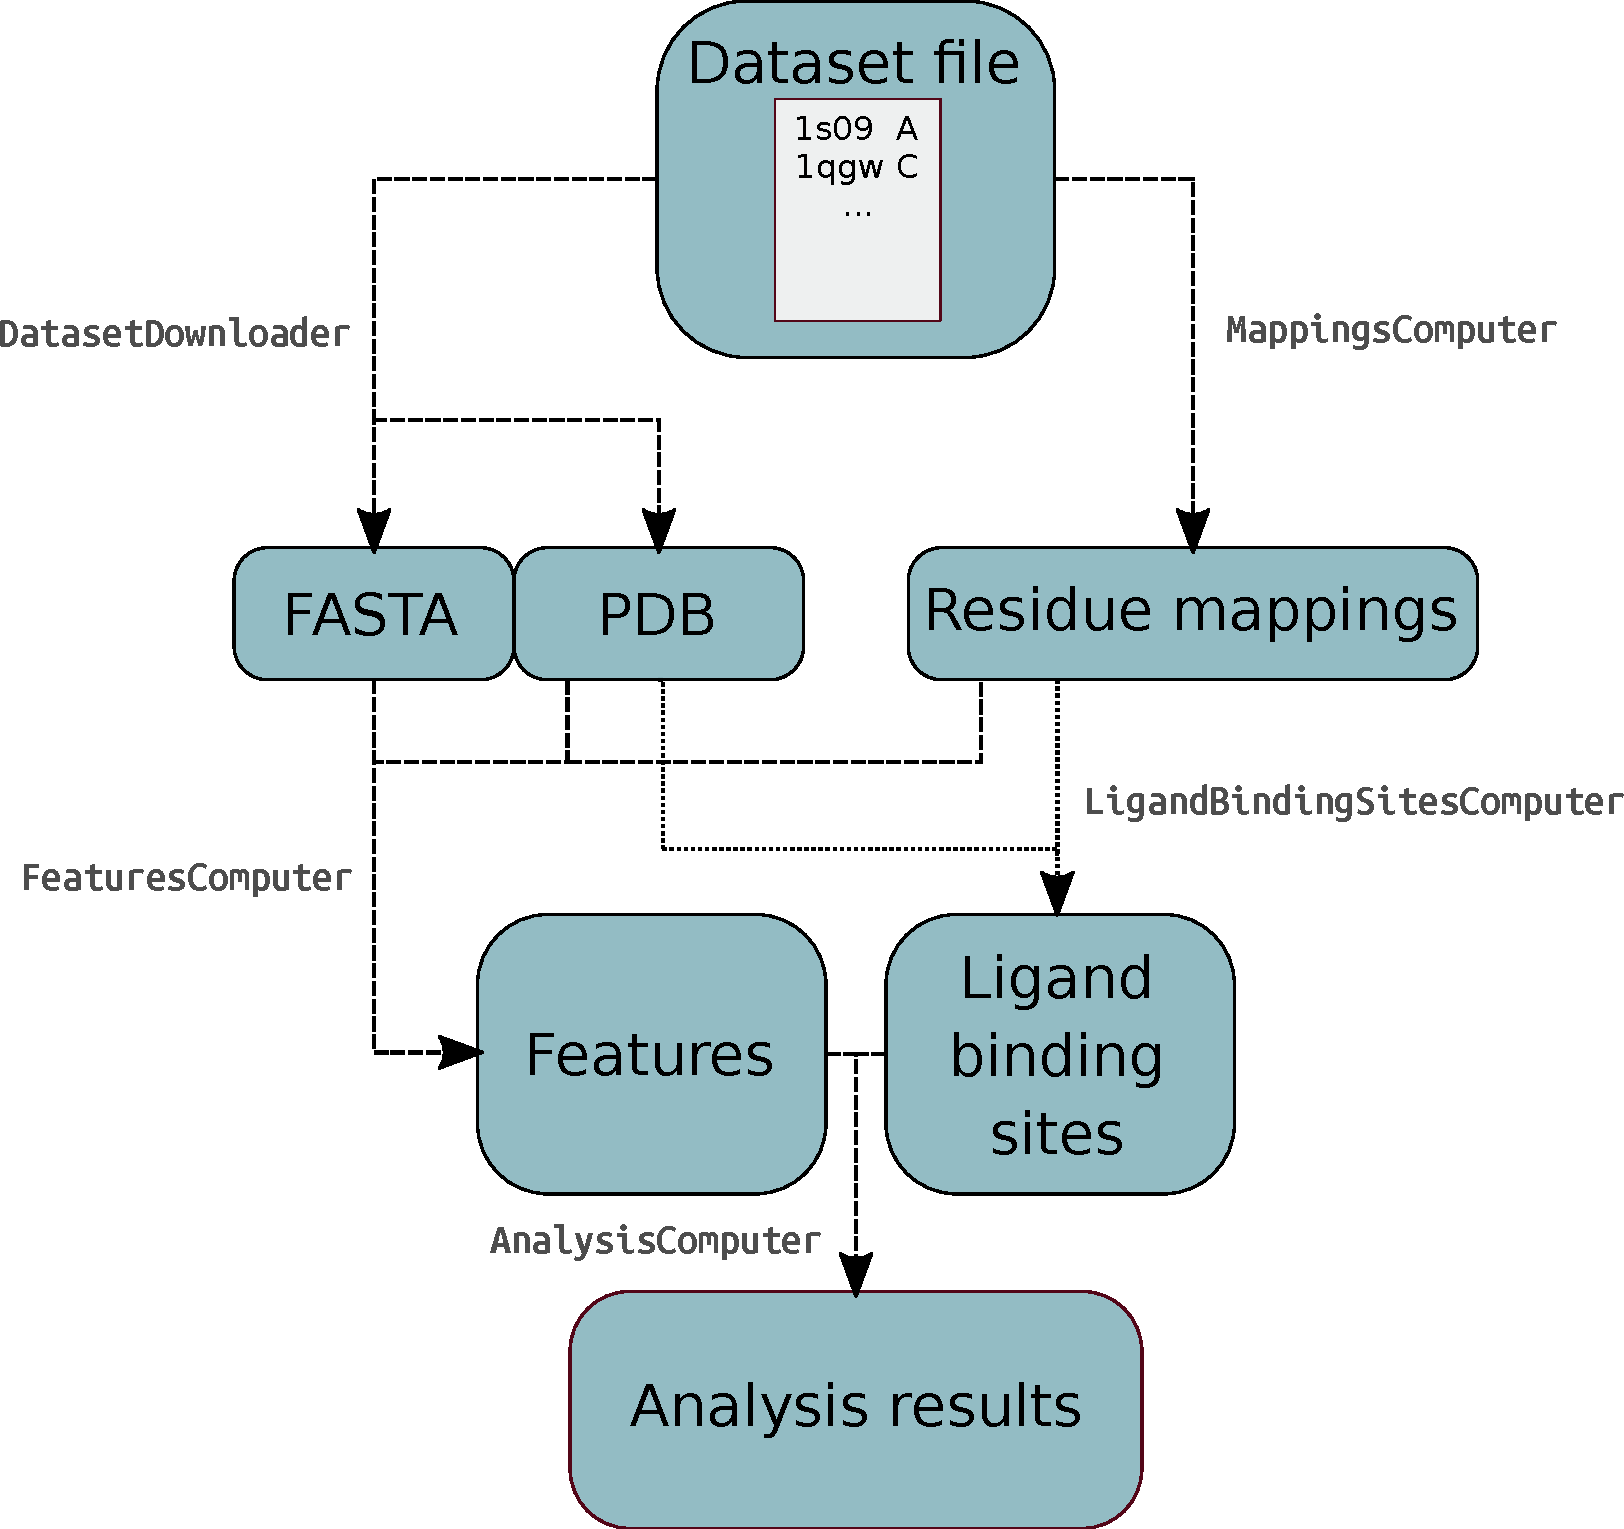
\includegraphics[width=120mm]{../img/pipelineDiagram.pdf}
\caption{Diagram of the pipeline structure.}
\label{fig:diagram}
\end{figure}

\section{Dataset file}
Dataset file is a mandatory input for the pipeline. It is a plain-text file with each row representing one structure. The columns are separated by whitespace. The first two columns are mandatory and they contain PDB ID and chain ID (pipeline can only work with single-chain structures). The third column is optional and it can define a comma-separated list of ligands which will be used for ligand binding sites computation.

\section{Data download}

For each structure, FASTA and PDB files are downloaded from PDBe, via Entry-based REST API \cite{pdbe_restapi}, which is one of the possibilities to access large amouts of data about individual PDB entries.

\section{Residue mappings}

Cross-referencing the protein structure with the primary sequence annotations, UniProt records and data from other resources would be very problematic without residue-level mappings.

The residues in the PDB files are assigned identifiers by the author, in order to match the identification used in the publication. The identifier of the residue is composed of two parts. The first one is a residue number, and the second one, called `insertion code', is usually a character. It is empty for most residues; it is usually used when there are insertions relative to the reference sequence. This numbering is used only in the PDB file and does not have to correspond with the primary sequence residues numbering. The author can assign the numbers how he or she desires; they do not have to start with one or zero, do not have to be in consecutive order and can even be negative. Furthermore, the PDB structure can cover only the part of the full-length sequence; it can even be split in parts, having some residues skipped.

For those reasons, the residue-level mappings are downloaded from PDBe REST API \cite{pdbe_restapi} at the beginning, they are cached in files and can be used whenever some values need to be mapped on the structure described in PDB.

For the cross-referencing between protein structures and protein sequences in UniProtKB \cite{uniprot}, we used UniProt segments mapping implemented in PDBe REST API. Mappings are assigned by the SIFTS \cite{sifts}, resource for the transfer of annotations between protein structure and sequence. The difference from the standard SIFTS  is that it uses the UniProt sequence as reference and thus, the output is a set of segments that reflects discontinuities in the UniProt sequence.

There is a presumable issue with UniProt segments - sometimes the returned segment does not have the same length in UniProt coordinates and PDB coordinates. It was reported and recognized as a bug, but unfortunately has not been corrected before running the experiments in this work; however, it is very rare and it concerns only a few structures; those were removed from the datasets. 

\section{Ligand binding sites labelling}

The assignment of labels non-binding/binding (0/1) is done directly according to the PDB file. The residue is labeled as binding if it has at least one non-hydrogen surface atom within distance 4.0 {\AA} of a non-hydrogen atom of any ligand. The distance 4.0 {\AA} can be changed with \texttt{-l} argument. This ligand-based definition of binding sites was used in previous large-scale study exploring the composition of binding sites \cite{lbscomposition}.

Only residues on the surface of the protein were taken into consideration in the analysis. The non-surface residues cannot be binding anyway, and excluding them decreases the imbalance between binding and non-binding residues counts. Furthermore, excluding the inner residues helps to reduce potential influence of  difference in feature value in surface vs. non-surface residues. For example, inner residues tend to be more hydrophobic in general. Thus, binding sites could seem to be more hydrophilic than non-binding sites, but it would not be clear whether it is not simply the effect of being on the surface of the protein.

The solvent-accessible surface was computed using \texttt{Bio.PDB.SASA} module in BioPython \cite{sasa}. It implements Shrake \& Rupley algorithm \cite{shrake} which uses a sphere of particular radius to probe the surface of the protein. It can be imagined as `rolling a ball' along the surface. The smaller the sphere radius, the more surface details it can detect. Fot this work, the default radius of 1.4 {\AA}, which approximates the radius of a water molecule, was used.

The algorithm computes the solvent accessible surface area of each residue. We defined the surface residues as residues that have less than 5\% of their surface accessible to the solvent. This cut-off was proposed by Miller \textit{et al.} \cite{sasaCutoff} and used in other studies\cite{jones,lbscomposition}. 

\section{Features}

This section describes all the implemented features and provides information on how to add user-defined features.

Pipeline can run only with a subset of implemented features, by listing them and passing as argument (e.g. \texttt{-f hydropathy,aromaticity}). If argument \texttt{-f} is not stated, all features defined in the config file are computed.

The config file is a file in JSON format that lists names of features, their type (binary, categorical, ordinal or continuous) and path to the class with implementation. Custom config file with user-defined features or with subsets of features can be created and passed as argument \texttt{-c new\_config\_path}.

TODO tabulka s prehledem featur, jejich jmena a typy, jestli jsou predikovane nebo pocitane atd.

\subsection{UniProtKB}

The UniProt Knowledgebase (UniProtKB) is a large database of well-annotated protein sequence data. It tries to achieve the minimal redundancy and it provides detailed, accurate and consistent annotations of the sequences \cite{uniprot}.

Sequence annotations (called `features') are available for every UniProtKB entry. They describe interesting sites and regions on the protein sequence and every feature has an associated description with more information, such as available evidence, source or related publications. The features are arranged in a well-organized manner on the website, in so called `Features viewer' with many overlapping tracks for different features. Nonetheless, for the purpose of this work, the best way to obtain the features was via the Proteins REST API \cite{proteins_api}. It provides the interface to  access the sequence annotation data as well as mapped variation data programmatically. The API is available at (\url{http://www.ebi.ac.uk/proteins/api/doc}) \cite{TODO}.

Features are classified into eight categories which are further subdivided into types. For example, the category `STRUCTURAL' comprises the types `HELIX', `TURN' and `STRAND'.

The types and categories that were chosen as potentially relevant for ligand binding sites prediction are described below.


\subsubsection{PTM}
Post-translational modifications are covalent chemical modifications of polypeptide chains after translation, usually modifying the functional group of the standard amino acids, or introducing a new group. They extend the set of the 20 standard amino acids and they can be important for the function of many proteins,as they can alter the interactions with other proteins, localization, activity, signal transduction, cell-cell interactions and other properties. Their enrichment in binding sites is very interesting to examine.

Three UniProtKB feature types were analysed: lipidation, glycosylation and type `MOD\_RES' which comprises phosphorylation, methylation, acetylation, amidation, formation of pyrrolidone carboxylic acid, isomerization, hydroxylation, sulfation, flavin-binding, cysteine oxidation and nitrosylation. Only experimentally determined modification sites are annotated, and they are further propagated to related orthologs when specific criteria are met \cite{mod_res}.

Since lipidaton and glycosylation data were very sparse (e.g. there were only 15 lipidation sites in the whole holo4k dataset composed of 3973 proteins), the fourth feature called `PTM' including all three types was added to the analysis.

\subsubsection{Disulfide bonds}
Another type of post-translational modifications are disulfide bonds formed between two cysteine residues. Both intrachain and interchain bonds are annotated by \mbox{UniProtKB}. The disulfide bonds may be either experimentally determined or predicted \cite{disulfid}.

\subsubsection{Non-standard residues}
Describes the occurence of non-standard amino acids (selenocysteine and pyrrolysine). There must be experimental evidence for this occurence; however, it can be propagated to close homologs \cite{non_std}.

\subsubsection{Secondary structure}
This feature category annotates three types of secondary structures: helices, beta sheets and hydrogen-bonded turns. Residues not belonging to any of the classes are in a random-coil structure. The `helix' class comprises alpha-helices, pi-helices and 3\textsubscript{10} helices.

The secondary structure assignment is made by DSSP algorithm \cite{dssp} based on the coordinate data sets extracted from the Protein Data Bank (PDB). They are neither predicted computationally, nor propagated to related species \cite{sec_str}.

\subsubsection{Natural variant}
This feature includes naturally occuring polymorphisms, variations between strains or RNA editing events \cite{natural_variant}.

\subsubsection{Variation}
\textit{Variation service} is a utility that can retrieve variation data from UniProtKB. The variants are either extracted from the scientific literature and manually reviewed, or mapped from large scale studies, such as 1000 Genomes \cite{1000genomes}, COSMIC \cite{cosmic}, ClinVar \cite{clinvar} or ExAC \cite{exac}. The Proteins REST API provides various options for variants retrieval, such as to filter by the consequence type, associated disease name, cross reference database type (e.g. ClinVar) or by the source type \cite{proteins_api}.


\subsubsection{Compositional bias}
The regions of compositional bias are parts of the polypeptide chain where some of the amino acids are over-represented, not following the standard frequencies. The regions can be enriched in one or more different amino acids \cite{https://www.uniprot.org/help/compbias}.



\subsection{PDBe-KB}
PDBe-KB (Protein Data Bank in Europe - Knowledge Base) is managed by the PDBe team at the European Bioinformatics Institute. It is a collaborative resource that aims to bring together the annotations from various sources and to show the macromolecular structures in broader biological context. 

One drawback of PDB is that every page represents only one entry that is based on a single experiment. There may be several PDB entries for the full-length protein, each covering only a segment of it. Nevertheless, the entries for the same protein are not interconnected. PDBe-KB has developed the \textit{aggregated views of proteins}, displaying an overview of all the data related to the full-length protein defined by the UniProtKB accession.

The structures from the PDB are extensively used by scientific software and other resources. There exist many valuable annotations, such as ligand binding sites, post-translational modification sites, molecular channels or effects of mutations, that are created outside of the PDB. The problem is that the data is fragmented and therefore it would require immense effort of a researcher to collect and make use of all available data for a structure of interest.

The aggregated views of proteins integrates the annotations from \textit{PDBe-KB partners}, collaborating scientific software developers. It facilitates the retrieval of these annotations with a uniform data access mechanism (via FTP or REST API). The project is called `FunPDBe'. A common data exchange scheme was defined to facilitate the transfer of data. \cite{pdbekb}

The use of PDBe-KB was difficult because of the lack of documentation and a few bugs that were encountered during this work (some of them corrected by now after pointing them out). However, it is understandable since it was launched only two years ago and the constant improvements are done since then.

\subsubsection{Conservation}
PDBe-KB provides pre-calculated residue-level conservation scores, obtained by a pipeline using HMMER and Skylign web servers that was described by Jakubec et al. \cite{3dpatch}.

The values of the score are integers ranging from 0 to 9, with 9 being the most conserved. Since scores higher than 4 were very sparse and the feature would not meet the assumptions of the Chi-squared test, the scores 4 and higher were merged into one category (4). This does not deteriorate the prediction nor the hypothesis test, as vast majority (over 95\%) of non-binding residues were scored 1 and lower.

\subsubsection{DynaMine}
DynaMine was developed by the Bio2Byte group \cite{bio2byte} and it is one of the PDBe-KB partner resources. It provides the annotations of the backbone dynamics predicted only from the FASTA sequence. DynaMine predicts backbone flexibility at the residue-level, using a linear regression model trained on a large dataset of curated NMR chemical shifts extracted from the Biological Magnetic Resonance Data Bank \cite{bmrb}. The predictor estimates the value of the `order parameter' (S\textsuperscript{2}) which is related to the rotational freedom of the N-H bond vector of the backbone. The values range from 0 (highly dynamic) to 1 (complete order) \cite{dynamine}.

\subsubsection{EFoldMine}
EFoldMine tool comes from the same group as DynaMine. It is a predictor of the early folding regions of proteins. It makes predictions at the residue-level derived only from the FASTA sequence. Internally it uses dynamics predictions and secondary structure propensities as features and the linear regression model is trained on data from NMR pulsed labelling experiments. Unfortunatelly, the early stages of protein folding are not understood very well so far and experimental data is very difficult to obtain. The predictor was trained on the dataset of only 30 proteins and its performance is quite poor \cite{efoldmine}.

\subsubsection{Depth}
Depth is a webserver that can measure residue burial within the protein. It is able to find small cavities in proteins and could be used as a ligand-binding sites predictor as such. The residue depth values are computed from the input PDB file.

The algorithm places input 3D structure in the box of model water, each residue with at least two hydration shells around itself. The water molecules in cavities are removed: the algorithm removes the water molecule if there are less than a given number of water molecules in its spherical volume of given size. The minimum number of neighbouring molecules and the spherical volume can be defined by the user. The removal is iterated until there are no more cavity waters. Residue depth is then computed as the distance to the closest water molecule \cite{depth}.


\subsection{PDB}

The following features can be computed or obtained directly from the PDB file.

\subsubsection{B factor}

The B factor, also called the Debye-Waller factor or the temperature factor, describes "the attenuation of X-ray or neutron scattering caused by thermal motion" \cite{bfactor}. It can be used to identify and interpret flexibility of proteins, supposing that high B factors are indicators of higher flexibility, whereas atoms with low B factors generally belong to the well-ordered parts of the structure. B factors can be also view as indicators of the relative vibrational motion of atoms in a protein \cite{bfactor}.

The values can be obtained directly from the PDB files: each ATOM record of a X-ray structure (except for hydrogens) deposited in PDB contains B factor value for the atom. B factor for a residue was computed be averaging B factors of all its atoms. 

\subsubsection{Contact number exposure}

Contact number (CN) is a simple solvent exposure measure that can be computed directly from the 3D structure. The CN value for residue is number of C$\alpha$ atoms within a sphere of chosen radius around the C$\alpha$ of that residue \cite{cn}.

The implementation in BioPython module \texttt{Bio.PDB.HSExposure} was used for computation, with default sphere radius 12 {\AA}.


\subsubsection{Half sphere exposure}

Half sphere exposure (HSE) is a solvent exposure measure introduced by Hamelryck (2005) \cite{hse}. The CN sphere (defined above) around the C$\alpha$ atom is split in two halves by the plane perpendicular to the C$\alpha$-C$\beta$ vector, going through the C$\alpha$. Two different measures are obtained, HSE-up, which is number of C$\alpha$ in `upper' half sphere (containing C$\beta$), and HSE-down, number of C$\alpha$ in the opposite sphere.

Class \texttt{HSExposureCB} from BioPython module \texttt{Bio.PDB.HSExposure} with default sphere radius 12 {\AA} was used. 

TODO obrazek?


\subsubsection{Phi and psi angles}

Three dihedral angles of a popypeptide backbone phi ($\phi$), psi ($\psi$) and omega ($\omega$) are depicted on the Figure~\ref{fig:angles}. While the $\omega$ angle is restricted due to the planar character of the peptide bond, the $\phi$ and $\psi$ angles have high rotational freedom around the N-C$\alpha$ ($\phi$ torsion) or C$\alpha$-C ($\psi$ torsion) bonds. The Ramachandran plot provides good visualization of the whole $\phi$\\$\psi$ space \cite{ramachandran}.
The angles sizes can be computed directly from the PDBe; for the purpose of this work, they were obtained from PDBe via REST API.

TODO obrazek vazby

\subsubsection{Cis peptide}

The majority of protein bonds is found with torsion angle $\omega$ close to 180$^\circ$, in so-called \textit{trans} conformation. The \textit{cis} isomer, having $\omega$ close to 0$^\circ$, is rather rare. The \textit{cis-trans} isomeration is involved in some biological processes, such as protein folding or membrane binding \cite{cispeptide}.

The residues with \textit{trans} bond are obtained from PDBe via REST API.


\subsection{FASTA}

There are features that can be derived directly from the FASTA sequence. Every amino acid is assigned a value and the feature values are obtained according to the FASTA file. These features are:

\begin{itemize}
\item \textbf{Hydropathy} - The values of hydropathy index proposed by J. Kyte and R. F. Doolittle \cite{kyte}. It takes into consideration hydrophilic and hydrophobic properties of the 20 amino acid side chains. It is based on experimental observations derived from the literature. It ranges from -4.5 (Arg) to 4.5 (Ile) and the larger the number is, the more hydrophobic the amino acid.
\item \textbf{Molecular weight} - Residue mass in Daltons.
\item \textbf{Polarity} - Classification of amino acids according to the side chain - categories Polar, Nonpolar and Polar uncharged.
\item \textbf{Charge} - Binary feature indicating whether the side group is charged in physiological pH.
\item \textbf{Aromaticity} - Binary feature labeling residues that contain aromatic ring.
\item \textbf{Hydrogen bond atoms} - Number of atoms of the side chain that are either hydrogen donor or hydrogen acceptor.
\end{itemize}

The biochemical properties of amino acids (all features above except hydropathy) were obtained from TODO citovat biochemie voet

\subsection{Other resources}

\subsubsection{MobiDB}

MobiDB is a database of protein disorder and mobility annotations. It provides annotations and predictions for intrinsically disordered (ID) proteins. MobiDB-lite is a method for highly specific predictions of long (at least 20 residues) disorders. It is a consensus-based prediction, combining results of eight different predictors
\cite{mobidb}. It has been integrated into the MobiDB and the web server provides programmatic access to retrieve single entries via REST API \cite{mobidbApi}.

\subsubsection{Conservation}

The sequence conservation scores for this feature are computed through Conservation pipeline \cite{conservation} implemented for P2Rank. The pipeline runs on local computer and needs to have SwissProt, UniRef90 and TrEMBL databases downloaded locally.

\subsection{User-defined features}

There are two ways to run the statistical analysis with user-defined features. The first, more time-demanding way is to compute all needed results (i.e. feature values and ligand binding sites labels) outside of the pipeline, and then run only the analysis task (with argument \texttt{-tasks A}). The data supplied to the pipeline need to be in the correct format; more details about the usage and a few  examples are described in the README file in the GitHub repository (\url{ https://github.com/katebrich/Master-thesis/tree/dev/Scripts} TODO).

Another, more straightforward possibility is to implement the new feature directly inside the pipeline. Two steps need to be made:

\begin{itemize}
\item to add the feature to the config file. The class with feature implementation is loaded dynamically according to the feature name, for the easier definition of new features,
\item to implement class with method \texttt{get\_values} which computes the feature values and returns them in the required format.
\end{itemize}

\section{Statistical analysis}

To find the features which are possibly important for prediction of protein-ligand binding sites, statistical analysis will have the crucial role. This section describes the method that was used to analyse the statistical significance of the features and to distinguish the ones that stand out in the known protein-ligand binding sites.

In this work, the problem will be seen as a hypothesis testing problem. Two populations will be compared: we take values of a feature for all the residues across all the proteins in the dataset and then compare the binding residues and non-binding residues.

The \textit{null hypothesis} and the \textit{alternative hypothesis}, denoted by $H_{0}$ and $H_{1}$, respectively, will be tested:

\begin{itemize}
\item \textbf{$H_{0}$} - The feature values in binding sites do not significantly differ from the values in non-binding sites.
\item \textbf{$H_{1}$} - There is a significant difference of feature values in binding sites and non-binding sites.
\end{itemize}

To decide which one of two complementary hypotheses is true, we employ a suitable \textit{hypothesis test}. Welch's test and Chi-squared test of indepence, both described below in more detail, will be used according to the feature type (binary, categorical or continuous). 

As one may expect, the tests are not error-proof and a mistake can be made in the decision of whether to accept or reject the null hypothesis. There are two types of errors in hypothesis testing, commonly known as \textit{Type I error} and \textit{Type II error}. The test has made a Type I error if it incorrectly rejects a true null hypothesis. If, on the other hand, a null hypothesis is accepted and it is not true, a Type II error has been made. Both situations are depicted in the Table~\ref{tab:hypothesis_testing_errors}. The ideal test would have both error probabilities equal to zero. Nevertheless, in most cases it is not possible to make both error probabilities arbitrarily small for a fixed sample size \cite{casella}.

\begin{table}[!htbp]
\centering
\renewcommand{\arraystretch}{2.5}
\begin{tabular}{l|l|c|c|}
\multicolumn{2}{c}{}&\multicolumn{2}{c}{\begin{large}Prediction \end{large}}\\
\cline{3-4}
\multicolumn{2}{c|}{}&Accept $H_{0}$&Reject $H_{0}$\\
\cline{2-4}
\multirow{2}{*}{\begin{large}Truth\end{large}}& \textbf{$H_{0}$} & \shortstack{Correct\\(true positive)} & \shortstack{\textbf{Type I error}\\(false positive)}\\
\cline{2-4}
& \textbf{$H_{1}$} & \shortstack{\textbf{Type II error}\\(false negative)} & \shortstack{Correct\\(true negative)} \\
\cline{2-4}
\end{tabular}
\caption{Type I and II Error in hypothesis testing.}\label{tab:hypothesis_testing_errors}
\end{table}

To control statistical significance of the result, we define a \textit{significance level}, a constant denoted by $\alpha$. It represents the probability  of making a Type I error, in other words, the probability that the study rejects the null hypothesis when it is true. The typical choices in practice are $\alpha =$ 0.01, 0.05 or 0.10 \cite{casella}. One should be aware that by fixing the significance level of the test, the experimenter is controlling only the Type I error probabilities. The probability of the Type II error is subject to factors such as the accuracy and completeness of the data and most importantly, the true effect size \cite{sham_purcell}. Our choice will be $\alpha =$ 0.05.

The \textit{P value} is reported as a result of the statistical test. The P value is the probability that, under the assumption the null hypothesis is true, we observe the same or greater difference between groups. Smaller values of $p(X)$ give stronger evidence for rejecting the null hypothesis. The null hypothesis is rejected when $p(X) \leq \alpha$. P value gives an idea of how strongly the data contradict the null hypothesis; furthermore, it allows other researchers to make a decision according to the significance level of their choice \cite{pvalue, sham_purcell, lehmann}.

\subsection{Implementation}

The following subsections rationalize the choice of Welch's and chi-squared test. The imlementation of these tests in module \texttt{scipy.stats} from the SciPy Python library \cite{scipy} was used in the pipeline; namely \texttt{ttest\_ind} with \texttt{equal\_var=False} to perform Welch's test, and \texttt{chi2\_contingency} for chi-squared test of independence.

By default, the pipeline computes the analysis for all the residues across all proteins in dataset. Neverthless, random sampling (without repetition) can be performed by specifying the sample size with argument \texttt{-s}. It is also possible to run more iterations of random sampling (argument \texttt{-i}). In this case, mean P values will be reported in summary. Individual P values from all iterations will be reported in separate files for each feature. Another possibility is to balance the number of binding and non-binding sites with argument \texttt{-b}. Same number of binding and non-binding residues will be sampled in that case.

The significance level is 0.05 by default and can be changed with \texttt{-a} argument.

The output of the whole analysis pipeline are folders with results for each feature, as well as several summary files:

\begin{itemize}
\item \textbf{p\_values\_means.csv} - Averaged P values obtained from all iterations.
\item \textbf{p\_values.csv} - List of P values from all iterations for all features. P values for individual features are also included in the results folder for each feature.
\item \textbf{p\_vals\_perc.csv} - Summary of how many percent of iterations had P value below given significance level $\alpha$ for each feature.
\item \textbf{means\_difference.csv} - Summary only for continuous features. Lists the differences of means and variances in both populations (all binding vs. all non-binding).
\item \textbf{binding\_ratios.csv} - binding/non-binding sites ratios for all iterations and all features.
\item \textbf{errors.txt} - Lists features that ended up with an error. This is often caused by lack of data (e.g. the sample size is bigger than number of rows or the data for a categorical feature are too sparse to meet the assumptions of Chi-squared test). Detailed information about the errors can be found in the log file.
\end{itemize}

The results folder for each feature contain file \texttt{pairs.txt} with paired ligand binding sites values and feature values, detailed information about all iterations, and various histograms and plots (according to the type of feature). 


\subsection{Welch's test}

Welch's unequal variances t-test, or Welch's test in short, is a two-sample hypothesis test used to decide whether two populations have different central tendencies (means or medians). The decision is made based on the samples from the two populations. It is a more robust alteration of the widely-used Student's t-test \cite{welch}.

Both Student's and Welch's t-test assume that the two examined populations follow a normal distribution \cite{welch}. Nevertheless, when testing for the equality of means of `large enough samples', the normality assumption can be violated thanks to the large sample theory and the Central Limit Theorem \cite{lehmann}. It has been shown in previous studies that for large samples, the statistical significance level is protected not only for normally distributed data, but also for many non-normal distributions; moreover, in case of Welch's test, this is true even for unequal variances \cite{zimmerman_zumbo_1993, zumbo_coulombe_1997, lumley}. According to  Lehmann and Romano \cite{lehmann}, the Type II error is also relatively insensitive to non-normality. Many articles and textbooks mention that when the sample sizes are small, nonparametric tests (i.e. tests that do not assume a specific distribution) such as the Mann-Whitney test \cite{mann} should be considered as an alternative to t-tests.
However, t-tests become superior when sample sizes increase \cite{zimmerman1998, lumley}. The simulations made by Lumley \textit{et al.} \cite{lumley} show that `sufficiently large sample size' means under 100 in most cases. Even for extremely non-normal data, the sufficient size is at most 500. This suggests that the choice of Welch's test is legitimate for this work.

The problem of the Student's t-test is that it performs badly when the variances of the two compared populations are unequal. Both Type I and Type II errors are negatively affected by violation of the equal variances assumption. The unequal variances can be less problematic if sample sizes are similar, but in practice, that is not always the case \cite{ruxton}.

Unlike Student's t-test, Welch's test does not assume equal variances of the populations. It performs well when the samples have unequal variances; furthermore, it can be used even when the samples have unequal sizes \cite{derrick}.

Some researchers tend to pre-test for variance equality by a preliminary test of variances (such as Levene's \cite{levene}, Bartlett's \cite{bartlett} or Brown-Forsythe test \cite{brown}) and then choose whether to use Student's or Welch's t-test. However, although this approach persists in some textbooks and software packages, it is not recommended by statisticians. As a preliminary test itself is subject to Type I and II errors, this two-stage procedure would not protect the significance level and could lead to incorrect decisions. One should be aware of the fact that even if the test suggested that the samples variances are nearly equal, it would not mean that the whole population variances could not differ to a larger extent \cite{zimmerman}. Some researchers may try to make the significance level of a preliminary test more strict, so that they could be more confident about the choice of the subsequent test; however, as the significance level decreases, the performance of the compound test paradoxically gets worse. According to Zimmerman \cite{zimmerman}, ``a higher Type I error rate of the preliminary test actually improves the performance of the compound test'' \cite{zimmerman}. This suggests that using the preliminary test is not correct in principle.

Welch's test should be used whenever the researcher is not sure that the variances are truly equal. Ruxton \cite{ruxton} even suggests the routine use of Welch's test. When the sample sizes and variances are equal, both tests perform similarly. When dealing with unequal variances and unequal sample sizes, Welch's test is more robust than Student's t-test and the Type I error rate does not deviate far from the nominal value \cite{derrick}. Hence, Welch's test can be applied without any significant disadvantages to Student's t-test.

For all the reasons stated above, Welch's test seems to be the best choice for the purpose of this study. It has the best combination of performance and ease of use, the calculation is straightforward and it is available in commonly used statistics packages. This test will be used for continuous features.

\subsection{Chi-squared ($\chi^{2}$) test of independence}

A different kind of tests will be needed for the analysis of categorical and binary features. In this section, the $\chi^{2}$ test will be compared to another well-known test for the analysis of data in contingency tables, the Fisher's exact test.

A \textit{contigency table} is a table displayed in a form of a matrix where cells represent a frequency distribution of samples in the categories. An example of a contingency table can be seen in Table~\ref{tab:contingency_table_example}. The sums of frequencies in rows and columns are called \textit{marginal totals}.

\begin{table}[!htbp]
\centering
\renewcommand{\arraystretch}{1.5}
\newcolumntype{s}{>{\columncolor{lightgray}} p{3cm}}
 \begin{tabular}{|c|c|c||c|} 
 \hline
  & Aromatic residue & Non-aromatic residue & Total \\ [0.5ex] 
 \hline
 Binding sites & 1016 & 4654 & 5670 \\ 
 \hline
 Non-binding sites & 4829 & 44545 & 49374 \\
 \hline\hline
 Total & 5845 & 49199 & 55044 \\
 \hline
\end{tabular}
\caption{A $2\times 2$ contingency table for binary feature \texttt{aromaticity} computed on dataset Chen11.}\label{tab:contingency_table_example}
\end{table}

The null hypothesis assumes independence of the groups; in our case, the assumption is that there is no difference in the proportions of the analysed feature between binding sites and non-binding sites.

Fisher's exact test belongs to a class of so-called \textit{exact tests}; it means that the P value is calculated accurately, not approximately, as is the case of many tests including Welch's test and $\chi^{2}$ test. Fisher's test is mostly used for $2\times 2$ contigency tables, although the principle of the computation can be extended to a general $m\times n$ table \cite{Mehta}. The principle of the test lies in computing the probability of obtaining a table that is more or equally extreme in the departure from the null hypothesis than the analysed table and has identical marginal totals \cite{bland}.

Chi-squared test if independence is able to decide whether the difference between the observed frequencies and the `expected frequencies' is statistically significant. The expected frequencies are computed for every cell as 
$\dfrac{row\: total\times column\:total}{grand\:total}$.
It can be imagined as the average frequencies we would get in the long run with the same marginal totals, assuming the null hypothesis is true (i.e. there is no association between groups). The result of the test tells how likely are we to observe given data under the assumption of the true null hypothesis \cite{bland}.

The biggest difference between the two mentioned tests is that the chi-squared test is based on a aproximation approach; therefore, it needs a `large enough' sample. W. G. Cochran (1952, 1954) proposed a set of recommendations about the minimum expectations to be used in $\chi^{2}$ tests and about the choice between Fisher's test and $\chi^{2}$ test:

\begin{itemize}
\item \textbf{The 2 x 2 table} - Fisher's exact test should be used whenever the sample size is smaller than 20, or when the sample size is smaller than 40 and if the expected frequency in at least one cell is less than 5. For sample sizes bigger than 40, always use chi-squared test \cite{cochran1952, cochran}.
\item \textbf{More than 1 degree of freedom} - Chi-squared test can be used when at most 20\% of cells have the expected frequency less than 5 and no cell have the expected frequencies less than 1 \cite{cochran1954}.
\end{itemize}

 These recommendations are presented in several textbooks and articles as a rule of thumb \cite{cochranRule} and recommended to be used in practice.

As the sample sizes in this work are very large, the number of binding and non-binding sites is unbalanced, and the data for some features can be sparse, chi-squared test is presumably better choice for both binary and categorical features.


\section{P2Rank models training and evaluation}





\chapter{Evaluation and results}


\section{Datasets}


The choice of datasets of protein-ligand complexes used for statistical analysis and P2Rank model training and evaluation was strongly inspired by the datasets described in the P2Rank article \cite{p2rank1}. The structures were re-downloaded directly from PDBe, according to their PDB ID (four-character alphanumeric identifier) and chain ID (one-character identifier) used in the original datasets. It was not possible to take the original datasets as they were, since the structures were not up-to-date and the annotations downloaded from the databases (e.g. feature values) could not be mapped properly.

Downloaded datasets were further checked and filtered: Obsolete structures were replaced with their current entries, structures that do not have a corresponding UniProt record were removed, as well as  structures with the incorrect segments mapping due to the bug in PDBe (mentioned in section TODO-ODKAZ).


The resulting datasets were named identically with the original datasets:

\begin{itemize}
  \item \textbf{Chen11}
  - a smaller non-redundant dataset that was originally designed for a comparative study of ligand binding sites predictors \cite{benchmark}. It comprises at most one representative chain for every SCOP family \cite{scop} to ensure the minimal sequence similarity and maximal variability in tertiary structure. The original dataset covers 6 structural classes, 148 protein folds, 184 superfamilies and 251 families \cite{benchmark}; after re-downloading and filtering, the numbers are slightly smaller.
  
  \item \textbf{Coach420}
  - a dataset that was originally taken from a benchmark study \cite{cofactor} and used in other studies \cite{coach, p2rank1}. The non-redundant dataset harbor mix of natural and drug-like ligand molecules.
  
  \item \textbf{Joined}
  - smaller datasets from previous studies merged together in one larger dataset. It comprises a set of drug-target complexes extracted from DrugBank, DrugPort and PDB DT198\cite{dt}, a benchmark set for the validation of protein-ligand docking performance \cite{astex}, and a dataset with bound and unbound structures used for evaluation of a ligand binding sites predictor \cite{ligsite}.
  
  \item \textbf{Holo4k}
  - a large set of protein-ligand complexes used in a large-scale evaluation of four binding sites predictors \cite{holo4k}.
\end{itemize}



TODO single chain

\subsection{Ligands filtering}

\section{Statistical analysis}

The statistical analysis of ligand binding sites properties was computed using the analysis pipeline described in TODO section 3 with default parameters. The results were collected for all the datasets, including the versions with filtered ligands. Let's set the significance level, denoted by $\alpha$, to 0.05.

Some features had to be excluded from the analysis, since the data were very sparse and the assumptions of the hypothesis tests would not be met. For example, there were only 15 lipidation sites in the whole holo4k dataset containing  857,635 residues. The excluded features are: \texttt{lipidation}, \texttt{glycosylation}, \texttt{non\_standard} and \texttt{compbias}

The \texttt{conservation} feature was computed only for the three smaller datasets and was omitted for holo4k. The computational time would be very high, as it takes 15-30 minutes on average per structure, and the dataset contains almost four thousand proteins. Nevertheless, the comparison on the other three datasets seems sufficient.

The problem with feature \texttt{variation} was that the data were missing for many structures (around 3/4) and downloading via REST API resulted in 404 Not Found error. Data are not available on the UniProt website either. This might be caused by lack of variation data from large-scale studies for some organisms. UniProt helpdesk was contacted to help to explain the issue, but unfortunately, the question was left without an answer. Nevertheless, the feature was analysed on the subset of structures where the data is available.

For some features downloaded from databases, such as \texttt{depth} or \texttt{dynamine}, there were missing data for a few structures as well. These cases were not very frequent and they most likely could not affect the analysis, so they were omitted.

Three artificial features were added for comparison and to check the validity of the tool:
\begin{itemize}
  \item \texttt{lbs} - Ligand binding sites labels (0/1). Should have the best performance of all the features, the P-value should be zero.
  \item \texttt{random\_binary} - Random binary numbers. Should not be significant.
  \item \texttt{random\_cont} - Random continuous feature with values from uniform distribution from 0 to 10.
\end{itemize}

The results for datasets without ligands filter are shown in Table~\ref{tab:pvaluesAll}. As we can see, most features appear to be statistically significant, having the P-value below the significance level $\alpha$. The results for the test features \texttt{lbs}, \texttt{random\_binary} and \texttt{random\_cont} seem to be okay. However, when looking at the histograms and plots, some results are not as expected. Let's take a look at the histogram depicted in Figure~\ref{fig:dynamine}: the distribution of \texttt{dynamine} values does not seem significantly different in binding and non-binding sites. Note that for better comparison of binding and non-binding sites (since their ratio is very unbalanced), the density is computed with respect to the number of binding or non-binding sites; the value in the histogram bin can be understood as conditional probability of getting that value when having a binding/non-binding residue.

% Please add the following required packages to your document preamble:
% \usepackage[table,xcdraw]{xcolor}
% If you use beamer only pass "xcolor=table" option, i.e. \documentclass[xcolor=table]{beamer}
\begin{table}[]
\centering
\begin{tabular}{lllll}
\hline
\textbf{}                     & \textbf{Chen11}                & \textbf{Coach420}               & \textbf{Joined}                & \textbf{Holo4k}                 \\ \hline
\textbf{lbs (test)}                  & 0                              & 0                               & 0                              & 0                               \\
\textbf{conservation}         & 0                              & 0                               & 0                              & ---                             \\
\textbf{pdbekb\_conservation} & 0                              & 0                               & 0                              & 0                               \\
\textbf{HSE\_up}              & 1.48E-266                      & 0                               & 0                              & 0                               \\
\textbf{exposure\_CN}         & 2.08E-240                      & 0                               & 0                              & 0                               \\
\textbf{depth}                & 1.63E-225                      & 3.37E-244                       & 0                              & 0                               \\
\textbf{bfactor}              & 6.57E-176                      & 1.02E-172                       & 9.03E-280                      & 0                               \\
\textbf{aa}                   & 2.43E-141                      & 4.01E-118                       & 2.09E-224                      & 0                               \\
\textbf{mol\_weight}          & 2.54E-141                      & 1.77E-117                       & 2.71E-225                      & 0                               \\
\textbf{HSE\_down}            & 4.23E-139                      & 6.18E-225                       & 0                              & 0                               \\
\textbf{hydropathy}           & 9.39E-136                      & 1.83E-118                       & 9.79E-222                      & 0                               \\
\textbf{aromaticity}          & 5.53E-79                       & 3.97E-56                        & 1.79E-102                      & 0                               \\
\textbf{H\_bond\_atoms}       & 3.59E-44                       & 2.89E-36                        & 4.50E-72                       & 0                               \\
\textbf{strand}               & 2.11E-17                       & 7.37E-32                        & 7.58E-36                       & 2.02E-252                       \\
\textbf{sec\_str}             & 2.88E-16                       & 1.57E-45                        & 4.91E-42                       & 0                               \\
\textbf{helix}                & 5.59E-06                       & 3.28E-29                        & 1.19E-26                       & 5.83E-279                       \\
\textbf{phi\_angle}           & 9.89E-06                       & 4.29E-05                        & 1.07E-07                       & 1.36E-42                        \\
\textbf{mobiDB}               & 0.0006394                      & 0.007984                        & 4.54E-06                       & 5.98E-51                        \\
\textbf{PTM}                  & 0.007131                       & 5.29E-05                        & 1.77E-15                       & 1.15E-104                       \\
\textbf{psi\_angle}           & 0.009603                       & 7.71E-16                        & 0.0009644                      & 1.30E-27                        \\
\textbf{charged}              & 0.009871                       & 4.38E-13                        & 2.99E-05                       & 2.53E-159                       \\
\textbf{dynamine}             & 0.0143                         & 0.02082                         & \cellcolor[HTML]{F54D4D}0.1595 & 1.70E-05                        \\
\textbf{efoldmine}            & 0.01699                        & 0.002727                        & 1.06E-09                       & 5.02E-07                        \\
\textbf{polarity}             & 0.02564                        & 9.01E-13                        & 3.11E-06                       & 4.18E-159                       \\
\textbf{variation*}            & \cellcolor[HTML]{F54D4D}0.1513 & \cellcolor[HTML]{F54D4D}0.07348 & \cellcolor[HTML]{F54D4D}0.698  & \cellcolor[HTML]{F54D4D}0.05166 \\
\textbf{cis\_peptide}         & \cellcolor[HTML]{F54D4D}0.2373 & 0.0001902                       & 4.44E-06                       & 3.46E-45                        \\
\textbf{disulfid}             & \cellcolor[HTML]{F54D4D}0.2753 & 1.82E-06                        & \cellcolor[HTML]{F54D4D}0.5603 & 1.71E-33                        \\
\textbf{natural\_variant}     & \cellcolor[HTML]{F54D4D}0.2793 & 0.02171                         & 2.14E-07                       & 3.39E-24                        \\
\textbf{mod\_res}             & \cellcolor[HTML]{F54D4D}0.3116 & 0.002696                        & 9.69E-05                       & 2.72E-49                        \\
\textbf{random\_cont (test)}         & \cellcolor[HTML]{F54D4D}0.4707 & \cellcolor[HTML]{F54D4D}0.706   & \cellcolor[HTML]{F54D4D}0.99   & \cellcolor[HTML]{F54D4D}0.1021  \\
\textbf{random\_binary (test)}       & \cellcolor[HTML]{F54D4D}0.5429 & \cellcolor[HTML]{F54D4D}0.922   & \cellcolor[HTML]{F54D4D}0.3561 & \cellcolor[HTML]{F54D4D}0.9322  \\
\textbf{turn}                 & \cellcolor[HTML]{F54D4D}0.8949 & 0.003081                        & \cellcolor[HTML]{F54D4D}0.7883 & 0.006317                        \\ \hline
\end{tabular}
\caption{P-values returned by hypothesis tests for individual features for all four datasets (without ligands filtering). Features are sorted according to the P-value in the first column. Values highlighted with red colour are higher that the chosen significance level $\alpha = 0.05$.\\\hspace{\textwidth}
*\texttt{variation} is computed only on the subsets of proteins for which the data were available in databases.}
\label{tab:pvaluesAll}
\end{table}

\begin{figure}[!htbp]
\centering
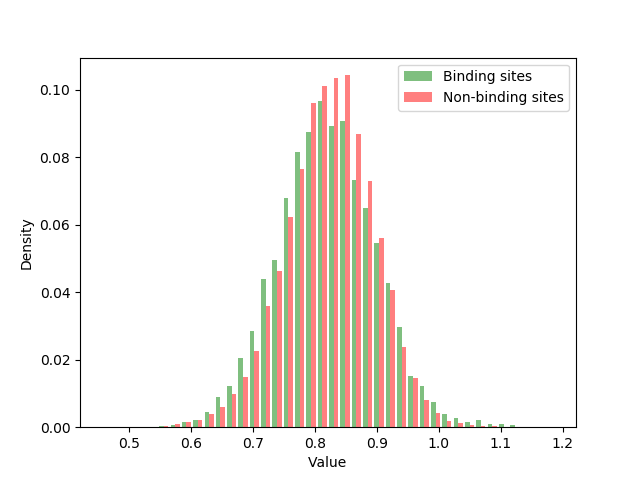
\includegraphics[width=120mm]{../img/dynamine_hist.png}
\caption{Histogram of feature \texttt{dynamine} computed on holo4k dataset. Density on the y-axis is computed with respect to the number of binding or non-binding sites. Difference in means: 0.0014; difference in variances: 0.0015.}
\label{fig:dynamine}
\end{figure}

One conspicuous thing about the Table~\ref{tab:pvaluesAll} is that, in general, the P-values are getting smaller as the dataset size grows (the datasets in the table are sorted from the smallest on the left to the largest on the right). This is referred to as the \textit{P-value problem}. For very large samples, the statistical power of hypothesis tests is higher, and causes P-value going to zero. When dealing with large samples, even the miniscule effects can become statistically significant. The test can detect subtler and more complex effects, which can be advantageous in some cases, but also misleading. It all depends on the purpose of the statistical testing. The question we should ask is not whether the results are statistically significant (which there almost always will be for large samples), but whether they are interesting for our research \cite{pvalueproblem}.

The P-value itself does not have an objective meaning and is not an unambiguous measure of evidence. The sample size hugely influences the significance, and relying only on the P-value can lead to acceptance of the hypothesis of no practical significance. Despite that, this appears to be a common practice. Lin et al. \cite{pvalueproblem} reviewed articles in two leading Information System (IS) journals and reported that 50\% of recent papers with sample sizes over 10,000 were relying on low P-values.

Let's see the P-value problem demonstated on our data. Figure~\ref{fig:pvalueDeflation} shows different speeds of P-value deflation for chosen features. At the first glance, the distributions of feature \texttt{exposure\_CN} in binding and non-binding sites differ, and sample size 25 is sufficient to get the P-value below significance level 0.05. On the other hand, \texttt{dynamine} does not seem to be relevant for the binding sites recognition, and yet, if the sample size is large enough, we get the significant result.


\begin{figure}[!htbp]
\centering
\begin{subfigure}[b]{\textwidth}
  \centering
  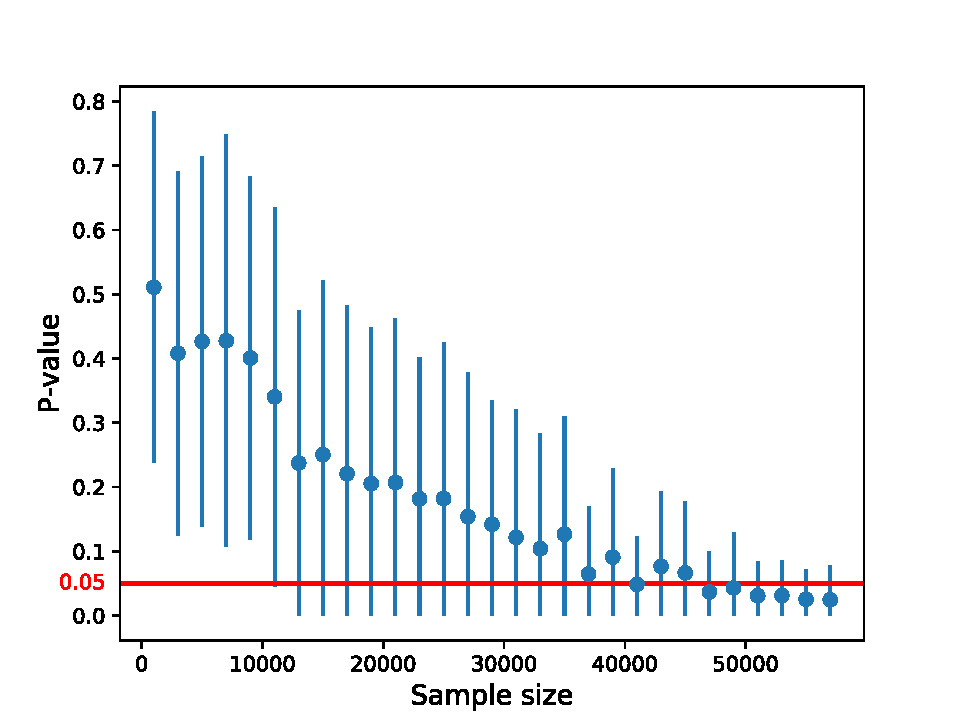
\includegraphics[width=0.475\linewidth]{../img/pValue_deflation_dynamine.pdf}%
  \hfill
  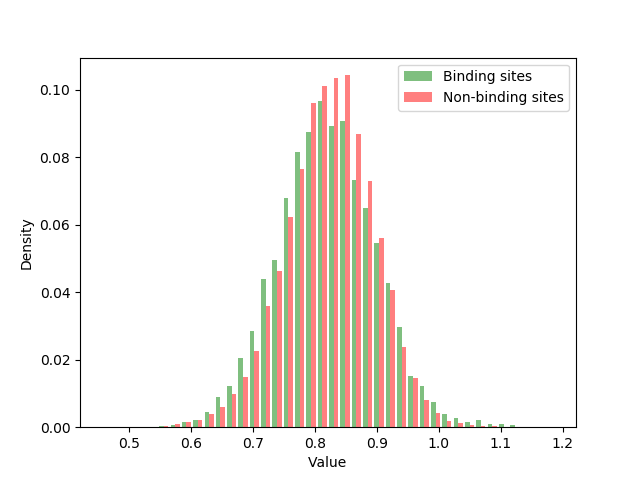
\includegraphics[width=0.475\linewidth]{../img/dynamine_hist.png}
  \caption{\texttt{dynamine}}
\end{subfigure}
\vskip\baselineskip
\begin{subfigure}[b]{\textwidth}
  \centering
  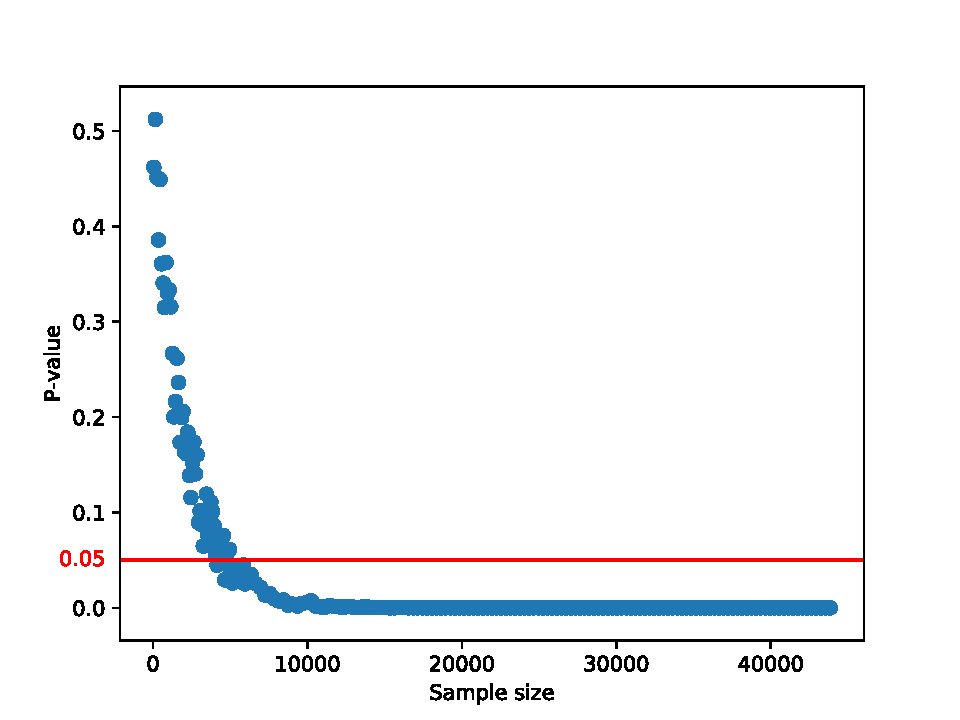
\includegraphics[width=0.475\linewidth]{../img/pValue_deflation_phi_angle.pdf}%
  \hfill
  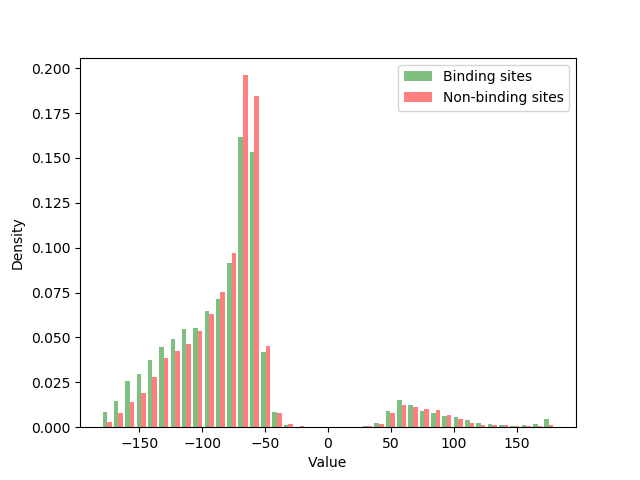
\includegraphics[width=0.475\linewidth]{../img/phi_angle_hist.png}
  \caption{\texttt{phi\_angle}}
\end{subfigure}
\vskip\baselineskip
\begin{subfigure}[b]{\textwidth}
  \centering
  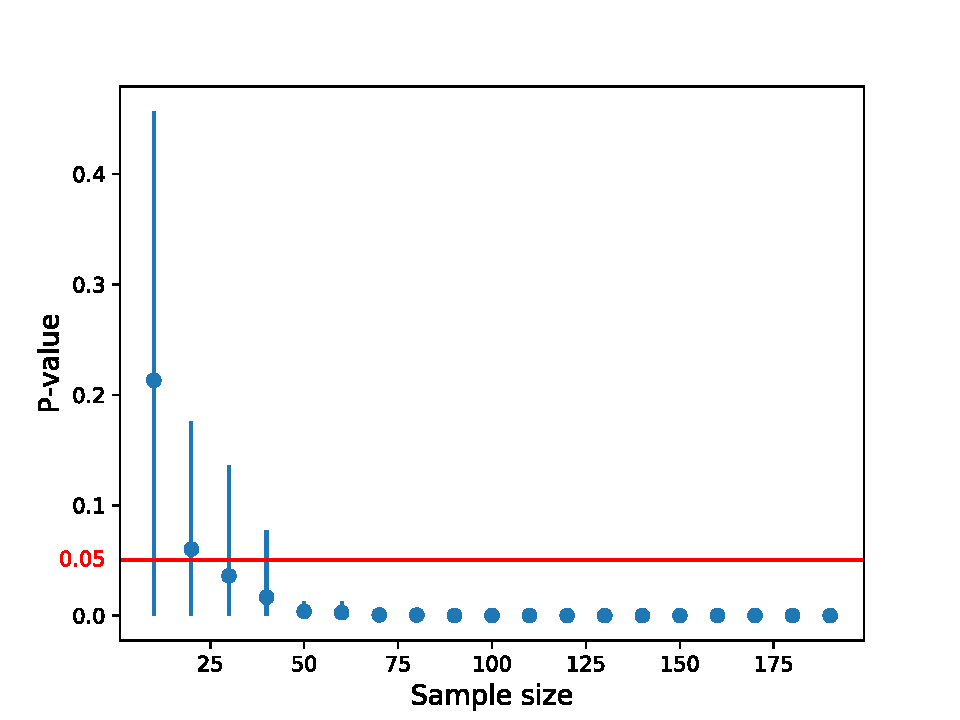
\includegraphics[width=0.475\linewidth]{../img/pValue_deflation_exposure_CN.pdf}%
  \hfill
  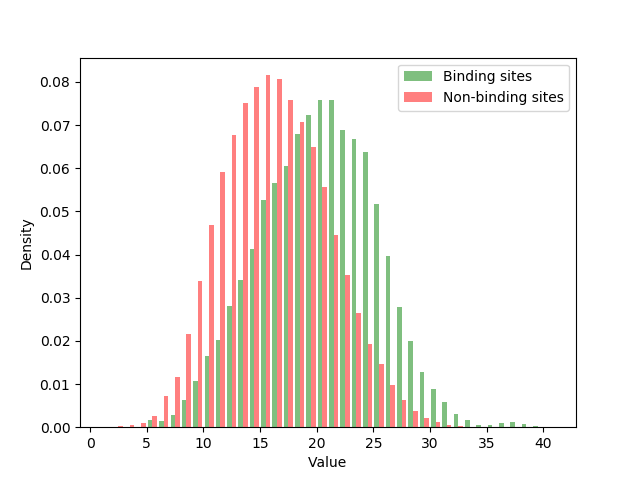
\includegraphics[width=0.475\linewidth]{../img/exposure_CN_hist.png}
  \caption{\texttt{exposure\_CN}}
\end{subfigure}
\caption{P-value deflation demonstrated on chosen features. The P-value decreases with increasing sample size. The speed of deflation is different for individual features. The y-axis shows mean P-values obtained from 100 iterations of random sampling with given sample size. The red line represents chosen significance level $\alpha=0.05$. }
\label{fig:pvalueDeflation}
\end{figure}


Therefore, the low P-values reported in Table~\ref{tab:pvaluesAll} are most likely mere artifacts of the large-sample sizes. Neverthleless, although P-value is not an objective measure of practical significance, it can be still used to compare the features relative to each other.

Another noticeable thing about Table~\ref{tab:pvaluesAll} is that the results for some features vary across datasets. Let's take a look at feature \texttt{turn}, for example. The P-value is very high for datasets Chen11 and Joined - even higher than P-values for the random features; contrarily, it is low for Coach420 and Holo4k. It is not true that the P-value would decrease with the increasing sample size. This leads to a question of how the datasets are composed, and whether they are representative samples from the whole population of proteins. Taken into consideration the way how the datasets were assembled, it is likely that some bias was introduced. The question is whether taking the whole PDB database would help to solve this issue. There probably would be the problem with redundancy of data, as close homologs and overlapping PDB entries would be included. Furthermore, the database itself is most likely a biased sample of the real world of proteins, as the tertiary structure is yet to be discovered for many of them. And most importantly, this approach would be computationally very demanding.

For the mentioned reasons, a different approach was implemented. Dataset `mix' was created by merging all four datasets together, removing a few duplicates. Random sampling without replacement was applied on this dataset, in each iteration taking a sample of 500 binding and 500 non-binding sites. 1000 iterations were computed and mean P-values were reported. The results are shown in Table~\ref{tab:pvalues500}. Note that the mean P-value cannot be understood in the original meaning of P-value. Nevertheless, the numbers provide relative comparison of the features.

The sample size of 500 was chosen for two reasons: firstly,  validity of the Central Limit Theorem needs to be assured, as described in section TODO. Lumley \textit{et al.} \cite{lumley} demonstrated that 500 is a sufficiently large sample even for extremely non-normal data. And secondly, the minimum sample size assuring the Central Limit Theorem validity should be chosen, to avoid the P-value problem. Smaller sample size would probably be sufficient for the Central Limit Theorem, as 500 is a very safe estimation. Nevertheless, the sample size could not be much smaller anyhow, since the data for some categorial features would be very sparse. Even with the sample size of 500, some features needed to be excluded from the analysis, as there was not sufficient number of positives in this smaller sample. TODO vyjmenovat je

% Please add the following required packages to your document preamble:
% \usepackage[table,xcdraw]{xcolor}
% If you use beamer only pass "xcolor=table" option, i.e. \documentclass[xcolor=table]{beamer}
\begin{table}[!htbp]
\centering
\begin{tabular}{llll}
\hline
                              & \textbf{no filter} & \textbf{P2Rank filter} & \textbf{MOAD filter} \\ \hline
\textbf{lbs (test)}                  & 1.33E-218          & 1.33E-218              & 1.33E-218            \\
\textbf{pdbekb\_conservation} & 3.55E-27           & 1.35E-30               & 4.43E-36             \\
\textbf{conservation}         & 1.11E-17           & 1.05E-27               & 7.86E-33             \\
\textbf{exposure\_CN}         & 4.72E-17           & 1.95E-21               & 1.30E-22             \\
\textbf{HSE\_up}              & 1.15E-14           & 2.15E-18               & 1.38E-18             \\
\textbf{depth}                & 8.00E-14           & 9.13E-16               & 2.83E-16             \\
\textbf{HSE\_down}            & 1.48E-09           & 1.59E-11               & 2.28E-11             \\
\textbf{bfactor}              & 2.56E-06           & 3.03E-08               & 3.97E-08             \\
\textbf{aa}                   & 0.006394           & 0.001172               & ---                  \\
\textbf{mol\_weight}          & ---                & 0.00129                & 0.002037             \\
\textbf{hydropathy}           & 0.00539            & 0.001376               & 0.001953             \\
\textbf{aromaticity}          & 0.02027            & 0.01516                & 0.02523              \\
\textbf{H\_bond\_atoms}       & 0.08081            & 0.02502                & 0.03019              \\
\textbf{charged}              & 0.2683             & 0.06663                & 0.08965              \\
\textbf{polarity}             & 0.2755             & 0.07131                & 0.1009               \\
\textbf{sec\_str}             & 0.133              & 0.0873                 & 0.02696              \\
\textbf{strand}               & 0.1491             & 0.1112                 & 0.04838              \\
\textbf{helix}                & 0.1361             & 0.1154                 & 0.02435              \\
\textbf{mobiDB}               & 0.3971             & 0.3844                 & 0.3653               \\
\textbf{phi\_angle}           & 0.3973             & 0.399                  & 0.3864               \\
\textbf{psi\_angle}           & 0.4213             & 0.4317                 & 0.2875               \\
\textbf{efoldmine}            & 0.4769             & 0.4373                 & 0.4839               \\
\textbf{dynamine}             & 0.4937             & 0.484                  & 0.4208               \\
\textbf{random\_cont (test)}         & 0.5029             & 0.5021                 & 0.4887               \\
\textbf{variation}            & 0.5387             & 0.5283                 & 0.5395               \\
\textbf{random\_binary (test)}       & 0.5374             & 0.5309                 & 0.5223               \\
\textbf{turn}                 & 0.5785             & 0.5982                 & 0.598                \\ \hline
\end{tabular}
\caption{Mean P-values computed from 1000 iterations of random sampling with sample size 500. Computed on dataset mix (4 datasets merged together) with three variations of ligands filtering. Features are sorted according to the P-value in the second column. Some values are missing because the assumptions of the test were not met.\\\hspace{\textwidth}
*\texttt{variation} is computed only on the subsets of proteins for which the data were available in databases.}
\label{tab:pvalues500}
\end{table}

The results for the datasets with different ligands filters does not seem to differ widely and does not reveal any additional informations. For that reason, following features analysis and computed plots will be shown only for the dataset `mix' with P2Rank ligands filter. The results obtained from the analysis pipeline for all the datasets and various sample sizes are included in the Attachments. TODO odkaz

The results for both conservation features \texttt{conservation} and \texttt{pdbekb\_conservation} turned out as expected. Sequence conservation has been used previously in many approaches for protein-ligand binding sites prediction and its importance for the prediction has been repeatedly demonstrated \cite{ligsite, cons, casp, prankweb}. The higher values of conservation for binding residues are clearly visible from the Figure~\ref{fig:conservation}.

\begin{figure}[!htbp]
\centering
\begin{subfigure}{.5\textwidth}
  \centering
  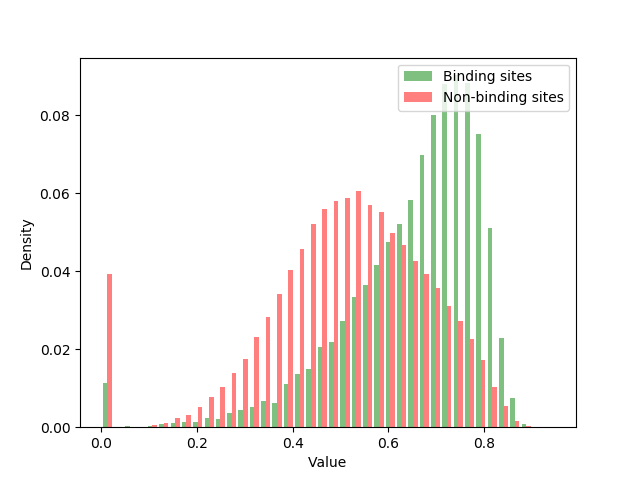
\includegraphics[width=1\linewidth]{../img/conservation_hist.png}
  \caption{\texttt{conservation}}
\end{subfigure}%
\begin{subfigure}{.5\textwidth}
  \centering
  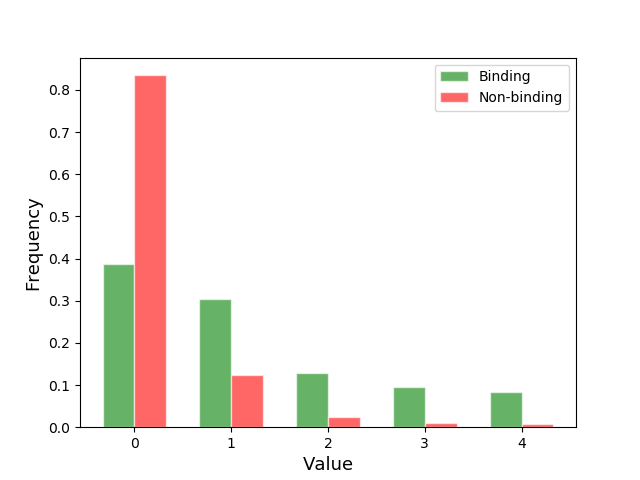
\includegraphics[width=1\linewidth]{../img/pdbekb_conservation_frequencies.png}
  \caption{\texttt{pdbekb\_conservation}}
\end{subfigure}
\caption{Higher values of conservation for binding residues demonstrated on two features: (a) continuous feature computed by the conservation pipeline, and (b) ordinal feature downloaded from PDBe-KB database.}
\label{fig:conservation}
\end{figure}

Features \texttt{HSE\_up}, \texttt{HSE\_down}, \texttt{exposure\_CN} and \texttt{depth} are closely related to the `buriedness' of the residue. Similarly as conservation, this feature was expected to be important for ligand binding sites recognition. Many binding sites are shaped as cavities, or concave pockets, on the surface of the 3D structure. The geometrical methods, such as LIGSITE \cite{ligsite} or PocketPicker \cite{pocketpicker}, as well as other approached, make use of this property. The histograms for these continuous features are depicted in Figure~\ref{fig:buriedness}


\begin{figure}[!htbp]
\centering
\begin{subfigure}{.5\textwidth}
  \centering
  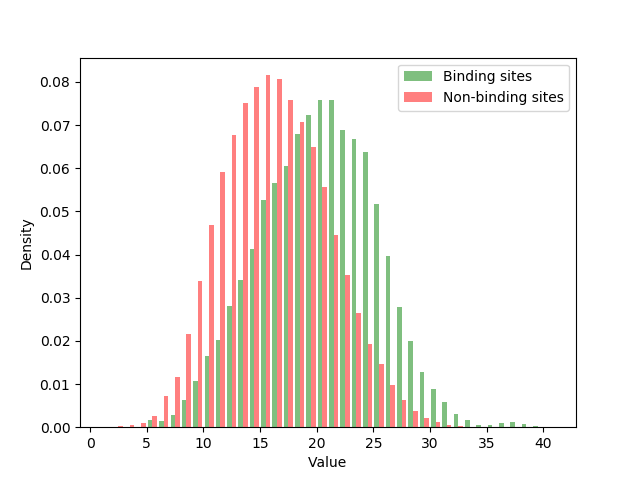
\includegraphics[width=1\linewidth]{../img/exposure_CN_hist.png}
  \caption{\texttt{exposure\_CN}}
\end{subfigure}%
\begin{subfigure}{.5\textwidth}
  \centering
  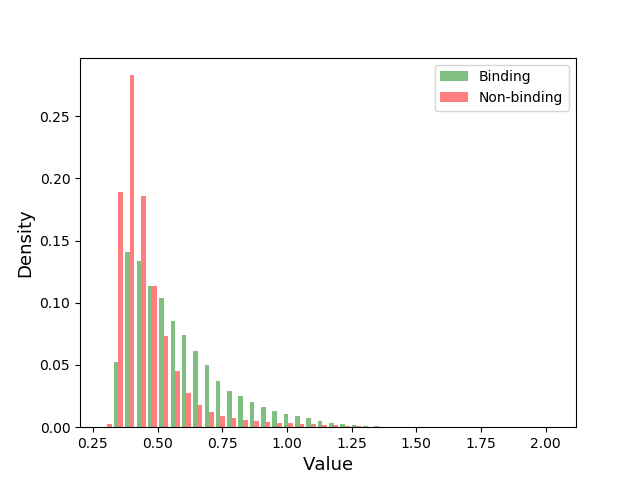
\includegraphics[width=1\linewidth]{../img/depth_hist.png}
  \caption{\texttt{depth}}
\end{subfigure}
\begin{subfigure}{.5\textwidth}
  \centering
  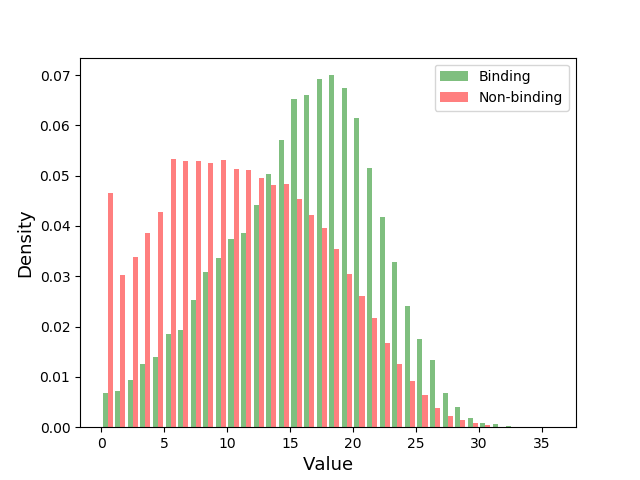
\includegraphics[width=1\linewidth]{../img/HSE_up_hist.png}
  \caption{\texttt{HSE\_up}}
\end{subfigure}%
\begin{subfigure}{.5\textwidth}
  \centering
  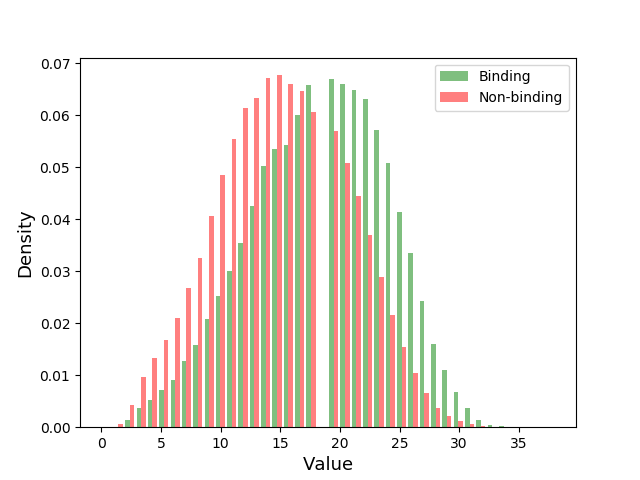
\includegraphics[width=1\linewidth]{../img/HSE_down_hist.png}
  \caption{\texttt{HSE\_down}}
\end{subfigure}
\caption{The features related with buriedness of the residue have higher values in binding sites.}
\label{fig:buriedness}
\end{figure}

The analysis reveals that binding sites have on average slightly lower B factor values (see Figure~\ref{fig:bfactor}). This suggests that binding sites are more well-ordered in general, whereas non-binding sites might have higher flexibility.

\begin{figure}[!htbp]
\centering
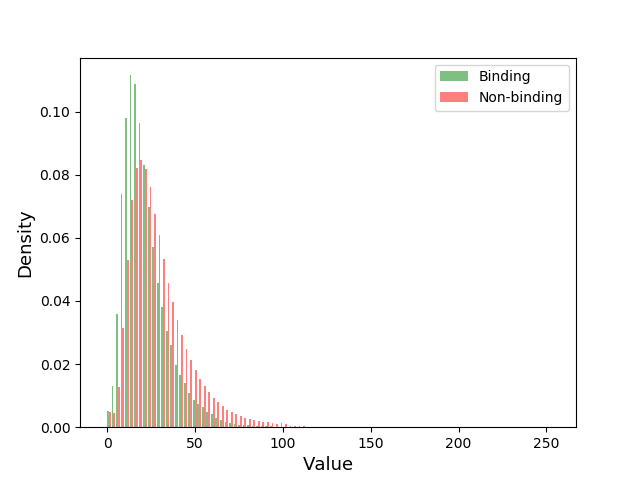
\includegraphics[width=0.7\linewidth]{../img/bfactor_hist.png}
\caption{\texttt{bfactor}: Binding sites have lower B factor values on average.}
\label{fig:bfactor}
\end{figure}

Binding and non-binding sites seem to have different residue composition. Let's take a look at Figure~\ref{fig:aa}. Cys, Trp, Phe, Tyr, Gly, His, Met and Ile all have high binding/non-binding ratios, and thus, are more likely to occur in binding sites. On the other hand, Pro, Glu, Gln, Lys and Asp disfavour binding sites. Arg, Val, Ser and Leu are very frequent in binding sites; however, they have the ratios similar to the total binding/non-binding ratio, as they are very frequent on the whole protein surface, not only in binding sites. This result is in accordance with a large-scale study that explored the composition of protein-ligand binding sites \cite{lbscomposition}. 
This is an interesting result and higher propensities of some amino acids to appear in binding sites could be used for their prediction.


\begin{figure}[!htbp]
\centering
\begin{subfigure}{\textwidth}
  \centering
  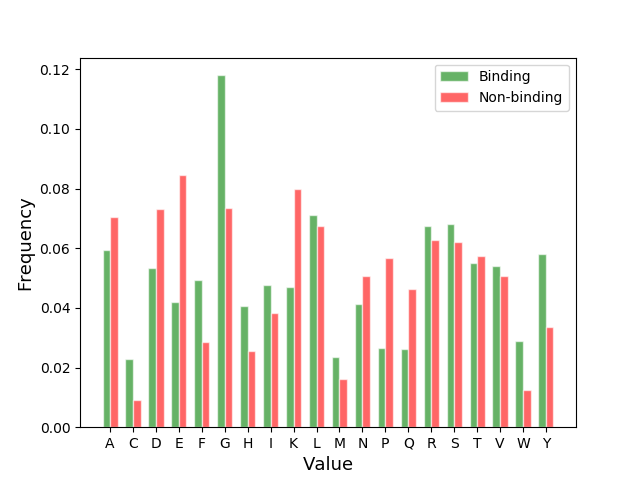
\includegraphics[width=0.7\linewidth]{../img/aa_frequencies.png}
  \caption{Frequencies of individual amino acids in binding and non-binding sites.}
\end{subfigure}
\begin{subfigure}{\textwidth}
  \centering
  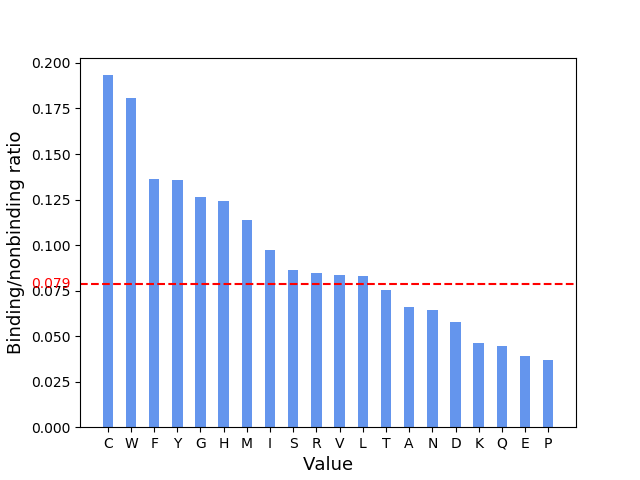
\includegraphics[width=0.7\linewidth]{../img/aa_ratios.png}
  \caption{Comparison of binding/non-binding ratios, computed as occurrences of the AA in binding sites divided by its occurrences in non-binding sites. The red line marks the total binding/non-binding ratio (total number of binding sites divided by total number of non-binding sites). High ratio means that the AA favours binding sites, and on the contrary, the low ratio indicates the tendency to occur in non-binding sites.}
\end{subfigure}
\caption{Feature \texttt{aa}.}
\label{fig:aa}
\end{figure}

TODO analyza nejakych dalsich featur?

TODO !!!!  It was discovered that high B-factor-characterized regions show a
higher average flexibility index, more pronounced average
hydrophilicity, and higher absolute net charge. - (11) Radivojac, P.; Obradovic, Z.; Smith, D. K.; Zhu, G.; Vucetic, S.;
Brown, C. J.; Lawson, J. D.; Dunker, A. K. Protein flexibility and
intrinsic disorder

TODO high-B-factor ordered regions
have a higher average flexibility index, a higher average
hydrophilicity, a higher average absolute net charge, and a
higher total charge than do either short or long disordered
regions. The low-B-factor ordered regions are significantly
enriched in hydrophobic residues and depleted in the total
number of charged residues compared to the other three
classes. 




\section{P2Rank models}

TODO evaluation metrics

The computed features were used to train new P2Rank models and analyze their practical significance. All models were trained with the same parameters as the default P2Rank model (100 trees, each grown with no depth limit using 6 features). The models were trained on the Chen11 dataset and evaluated on Coach420 dataset. The training was done with parameter \texttt{loop=10} which means that training was done 10 times, every time with different random seed, and the performance of the 10 resulting models was averaged at the end. This is important for the comparison of features importance so that the random behaviour of the random forest classifier does not have such big influence.

The features obtained by the analysis pipeline are called `csv features' in the following section, in accordance with the terminology used by P2Rank for user-defined features in csv files.

TODO ze se nektere featury vynechaly a proc: aa, secstr, variation

The performance of the baseline model (all default P2Rank features and no csv feature) was compared with the model trained on all csv features (without test features \texttt{lbs}, \texttt{random\_binary} and \texttt{random\_cont}), and the model trained with all P2Rank features and all csv features. The results are summarized in Table~\ref{tab:p2rankbaseline}. Our baseline model performs a little better in the Top-n category than the default P2Rank model described in the P2Rank article \cite{p2rank1}, which achieves the success rate of 72\%. This can be caused by  slightly different datasets, as described in Section TODO, or simply by the random behaviour of the classifier.

The performance of the model trained on the csv features is inferior to the baseline model, but surprisingly, the difference is very small. The reason probably is that many features used by P2Rank are identical or very similar to the new csv features. P2Rank already used B factor, amino acid properties, buriedness and other properties for training, and csv features evidently does not contribute with much new information. That is visible on the model with both csv and P2Rank features: the performance is superior only by 1.5\%. Moreover, csv features are mutually correlated, as well as P2Rank features. 

\begin{table}[]
\centering
\begin{tabular}{lll}
\hline
\textbf{}                                 & Top-n & Top-(n+2) \\ \hline
\textbf{P2Rank features (baseline model)} & 73.6  & 78        \\
\textbf{csv features}                     & 70.7  & 73.9      \\
\textbf{P2Rank + csv features}            & 75.1  & 77.5      \\ \hline
\end{tabular}
\caption{Comparison of the performance of models with different sets of features.}
\label{tab:p2rankbaseline}
\end{table}

Let's take a look at how the csv features help to improve the performance when adding only one of them at a time. Table~\ref{tab:p2rankCSV} summarizes the results of training one model per feature, with all P2Rank default features plus given csv feature. Models with features \texttt{pdbekb\_conservation} and \texttt{conservation} are clearly superior to the baseline model.  There are other features that perform better than the baseline model by tenths of percent; nevertheless, this difference is too small to proclaim the results significant. Although there are features that are enriched in binding sites, as has been shown previously, they do not help to improve P2Rank performance, probably due to the correlations and recurrence of the same features.

\begin{table}[]
\centering
\begin{tabular}{lll}
\hline
                              & Top-n & Top-(n+2) \\ \hline
\textbf{lbs (test)}                  & 90.2  & 90.5      \\
\textbf{pdbekb\_conservation} & 78.9  & 81.6      \\
\textbf{conservation}         & 76.8  & 79.8      \\
\textbf{HSE\_down}            & 74.1  & 78.6      \\
\textbf{helix}                & 73.6  & 78.6      \\
\textbf{psi\_angle}           & 74.3  & 78.4      \\
\textbf{depth}                & 73.2  & 78.4      \\
\textbf{turn}                 & 73.8  & 78.3      \\
\textbf{HSE\_up}              & 73.6  & 78.2      \\
\textbf{strand}               & 73.6  & 78.2      \\
\textbf{mol\_weight}          & 73.5  & 78.2      \\
\textbf{aromaticity}          & 73.6  & 78.1      \\
\textbf{dynamine}             & 73.6  & 78.1      \\
\textbf{charged}              & 73.5  & 78.1      \\
\textbf{H\_bond\_atoms}       & 73.5  & 78.1      \\
\textbf{efoldmine}            & 74.1  & 78        \\
\textbf{phi\_angle}           & 73.8  & 78        \\
\textbf{mobiDB}               & 73.6  & 78        \\
\textbf{exposure\_CN}         & 73.5  & 78        \\
\textbf{hydropathy}           & 73.3  & 77.8      \\
\textbf{bfactor}              & 73    & 77.5      \\ \hline
\end{tabular}
\caption{Performance of models trained with all P2Rank features plus one extra csv feature at a time. The features are sorted according to the performance in Top-(n+2) category.}
\label{tab:p2rankCSV}
\end{table}

In another experiment, all P2Rank features were switched off and the models were trained with csv features only, one at a time. The performances are of course wery poor, but it gives us the relative comparison of csv features, without the effect of correlation with existing P2Rank features. Table~\ref{tab:p2rankCSVOne}


\begin{table}[]
\centering
\begin{tabular}{lll}
\hline
                              & Top-n & Top-(n+2) \\ \hline
\textbf{lbs (test)}                  & 88.3  & 90        \\
\textbf{pdbekb\_conservation} & 57.1  & 71.9      \\
\textbf{HSE\_up}              & 36.7  & 52.1      \\
\textbf{conservation}         & 34    & 49.7      \\
\textbf{exposure\_CN}         & 30.8  & 44.7      \\
\textbf{HSE\_down}            & 28.2  & 41.8      \\
\textbf{depth}                & 25.5  & 37.5      \\
\textbf{aromaticity}          & 14.3  & 25.5      \\
\textbf{dynamine}             & 10.6  & 17.7      \\
\textbf{phi\_angle}           & 8.7   & 16.3      \\
\textbf{hydropathy}           & 10.7  & 16        \\
\textbf{mol\_weight}          & 8.4   & 15.7      \\
\textbf{efoldmine}            & 7.2   & 13.5      \\
\textbf{strand}               & 6.3   & 10.9      \\
\textbf{psi\_angle}           & 5.8   & 9.8       \\
\textbf{bfactor}              & 4.2   & 6.1       \\
\textbf{helix}                & 3.9   & 6         \\
\textbf{charged}              & 3.6   & 5         \\
\textbf{H\_bond\_atoms}       & 3.3   & 4.9       \\
\textbf{mobiDB}               & 2.4   & 4.7       \\
\textbf{turn}                 & 0     & 0         \\ \hline
\end{tabular}
\caption{Sorted by sec col}
\label{tab:p2rankCSVOne}
\end{table}


\chapter*{Conclusion}
\addcontentsline{toc}{chapter}{Conclusion}


Conclusion.

%%% Abbreviations used in the thesis, if any, including their explanation
%%% In mathematical theses, it could be better to move the list of abbreviations to the beginning of the thesis.
\chapwithtoc{List of Abbreviations}
\begin{tabular}{ll}
AA & Amino acid \\
atd & a tak dale \\
\end{tabular}


%%% Bibliography
%%% Bibliography (literature used as a source)
%%%
%%% We employ bibTeX to construct the bibliography. It processes
%%% citations in the text (e.g., the \cite{...} macro) and looks up
%%% relevant entries in the bibliography.bib file.
%%%
%%% The \bibliographystyle command selects, which style will be used
%%% for references from the text. The argument in curly brackets is
%%% the name of the corresponding style file (*.bst). Both styles
%%% mentioned in this template are included in LaTeX distributions.

\bibliographystyle{plainnat}    %% Author (year)
%\bibliographystyle{unsrt}     %% [number] unsrt

\renewcommand{\bibname}{Bibliography}

%%% Generate the bibliography. Beware that if you cited no works,
%%% the empty list will be omitted completely.

\bibliography{bibliography}

%%% If case you prefer to write the bibliography manually (without bibTeX),
%%% you can use the following. Please follow the ISO 690 standard and
%%% citation conventions of your field of research.

% \begin{thebibliography}{99}
%
% \bibitem{lamport94}
%   {\sc Lamport,} Leslie.
%   \emph{\LaTeX: A Document Preparation System}.
%   2nd edition.
%   Massachusetts: Addison Wesley, 1994.
%   ISBN 0-201-52983-1.
%
% \end{thebibliography}


%%% Figures used in the thesis (consider if this is needed)
%\listoffigures

%%% Tables used in the thesis (consider if this is needed)
%%% In mathematical theses, it could be better to move the list of tables to the beginning of the thesis.
%\listoftables



%%% Attachments to the bachelor thesis, if any. Each attachment must be
%%% referred to at least once from the text of the thesis. Attachments
%%% are numbered.
%%%
%%% The printed version should preferably contain attachments, which can be
%%% read (additional tables and charts, supplementary text, examples of
%%% program output, etc.). The electronic version is more suited for attachments
%%% which will likely be used in an electronic form rather than read (program
%%% source code, data files, interactive charts, etc.). Electronic attachments
%%% should be uploaded to SIS and optionally also included in the thesis on a~CD/DVD.
%%% Allowed file formats are specified in- provision of the rector no. 72/2017.
\appendix
\chapter{Attachments}

The attached CD contains two attachments:

\section{attachment1}

blabla

\section{attachment2}

blabla

\openright
\end{document}